% !TeX root = ../main.tex
% !TEX root = ../main.tex
% -*- root: ../main.tex -*-
% -*- program: pdflatex -*-
\chapter{利用样条插值方法方法对~MRPC~进行刻度}

~MRPC-TOF~直接测量的信息包括原始的飞行时间和过阈时间(~time-over-threshold~,简称~TOT~)。为了得到精确的飞行时间信息,还需要对时幅游走、过大信号、粒子在对数条上的传播时间,以及在电子学电缆等的时间延迟等因素进行刻度和修正,还要进行离线分析。为了得到良好的时间分辨,必须对不同粒子的样本进行离线的刻度和修正,得到相应的刻度常数,再对原始数据进行重建从而得到飞行时间探测器的性能。
%\begin{comment}
~MRPC-TOF~的离线刻度是通过比较测量时间~$t_{mea}=t_{raw}-t_{0}-t_{cor}$~与带电粒子从对撞顶点到击中~MRPC-TOF~的预期飞行时间~$t_{exp}=L/\beta c$~来比较,其中~$t_{0}$~是事例的起始时间,~$t_{cor}$~是时间的修正项;~c~是真空中的光
速,$\beta=p/\sqrt{p^2+m^2}$是带电粒子的飞行时间,~m~是粒子的质量,飞行长度~L~和动量~P~是通过主漂移室(~MDC~)测量得到的。飞行时间修正项~$t_{cor}$~是过阈时间~TOT~和~Z~向击中位置的函数。
%\end{comment}
对于每一个读数条,每个读出单元定义:
%\begin{equation}
\begin{displaymath}
\chi^2(counter,readout)=\sum\limits_{event}(t_{mea}-t_{exp})^2
\end{displaymath}
%\end{equation}
通过分析大量的事例样本,进行反复迭代,利用最小~$\chi^2$~方法,刻度常数项可以通过~$\partial\chi^2/\partial P_{i}=0$~得到。在重建中,利用刻度得到的刻度常数对原始的飞行时间信息进行重建,就可以得到经过刻度修正得到的飞行时间信息。

STAR~实验MRPC采用的是样条插值(~spline Fit~)刻度的方法。因此本文也对~BESIII~的~MRPC~进行了样条插值方法的研究。
本章主要介绍样条插值方法。分两部分介绍:先对~TOT~进行插值,之后对击中位置~Z~修正;先对击中位置~Z~进行修正,之后对~TOT~进行插值。并进行了一定的结果比较,发现先修正~Z~,然后对~TOT~进行插值的结果比另一种方法好。

样条插值方法优点:光滑性好,且低阶就能拟合的很好。高能所集群下的~root~中有关于~TSpline~的类包,可以利用它完成样条插值的拟合。

本章数据选用的是~160524-160530~这期间~BESIII~对撞数据中的~Bhabha~事例。选用~Bhabha~事例是因为它事例量大,易于挑选,纯度高,适合做刻度样本。

%%%%%%%%%%%%%%%%%%%%%%%%%%%%%%%%%%%%%%%%%%%%%%%%%%%%%%%%%%%%%%%%%%%%%%%%%%%%%%
\section{修正~Z~前进行插值}
%%%%%%%%%%%%%%%%%%%%%%%%%%%%%%%%%%%%%%%%%%%%%%%%%%%%%%%%%%%%%%%%%%%%%%%%%%%%%%

本节以挑选的~Bhabha~事例中击中位置在~MRPC~中模块编号为~55~,对数条编号为~7~这一个对数条为例。具体做法,就是先对~TOT~进行插值修正,之后对得到的结果再次对~Z~进行修正得到最终的时间分辨等刻度信息。
\subsection{等事例数分~bin~拟合}
\begin{itemize}
    \item 以TOT的大小为度量对所选的事例数进行等事例数分~bin~
    \item 对于每个~bin~区间,进行拟合
    \item 对于上一步得到的~mean~值进行插值,得到插值的刻度常数
    \item 利用上一步得到的刻度常数,对时间信息进行修正 
\end{itemize}
等事例数分~bin~的原因是时间随~TOT~的分布是不均匀的。在小~q~(声明:以下所有出现~q~都等同于~TOT~)和大~q~部分事例数很少,如果采用等区间分~bin~的话,会出现比较大的误差棒。分~bin~完成后,发现一个~bin~内时间有两个峰值。图~\ref{fig:ScatterDiagram}~是时间对~TOT~的分布,图~\ref{fig:cutScatterDiagram}~是图~\ref{fig:ScatterDiagram}~截取的一部分。

\begin{figure}[htbp]
\begin{minipage}[t]{0.5\linewidth}
%\centering
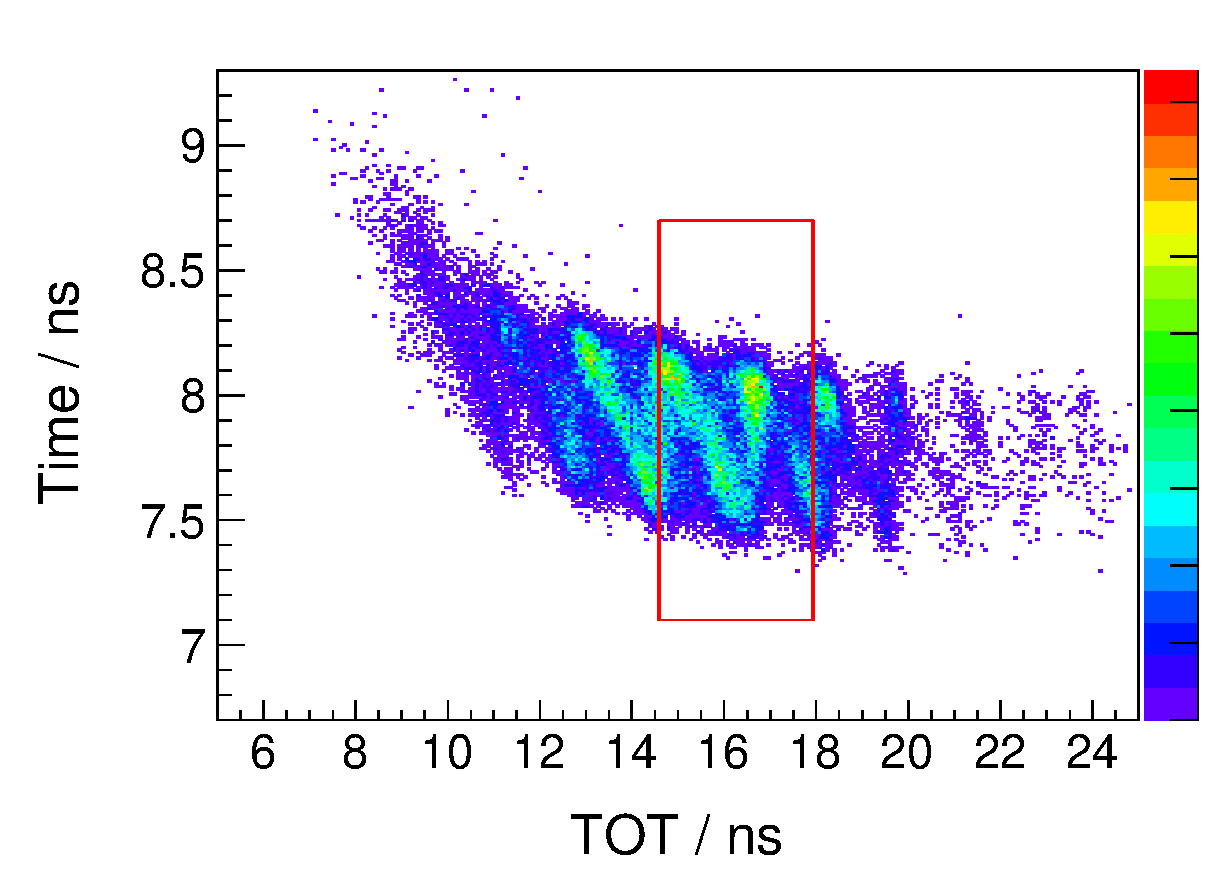
\includegraphics[width=0.9\textwidth]{chap2/ScatterDiagram.eps}
\subcaption{时间对TOT的分布}
\label{fig:ScatterDiagram}
\end{minipage}%
\hfill
\begin{minipage}[t]{0.5\linewidth}
%\centering
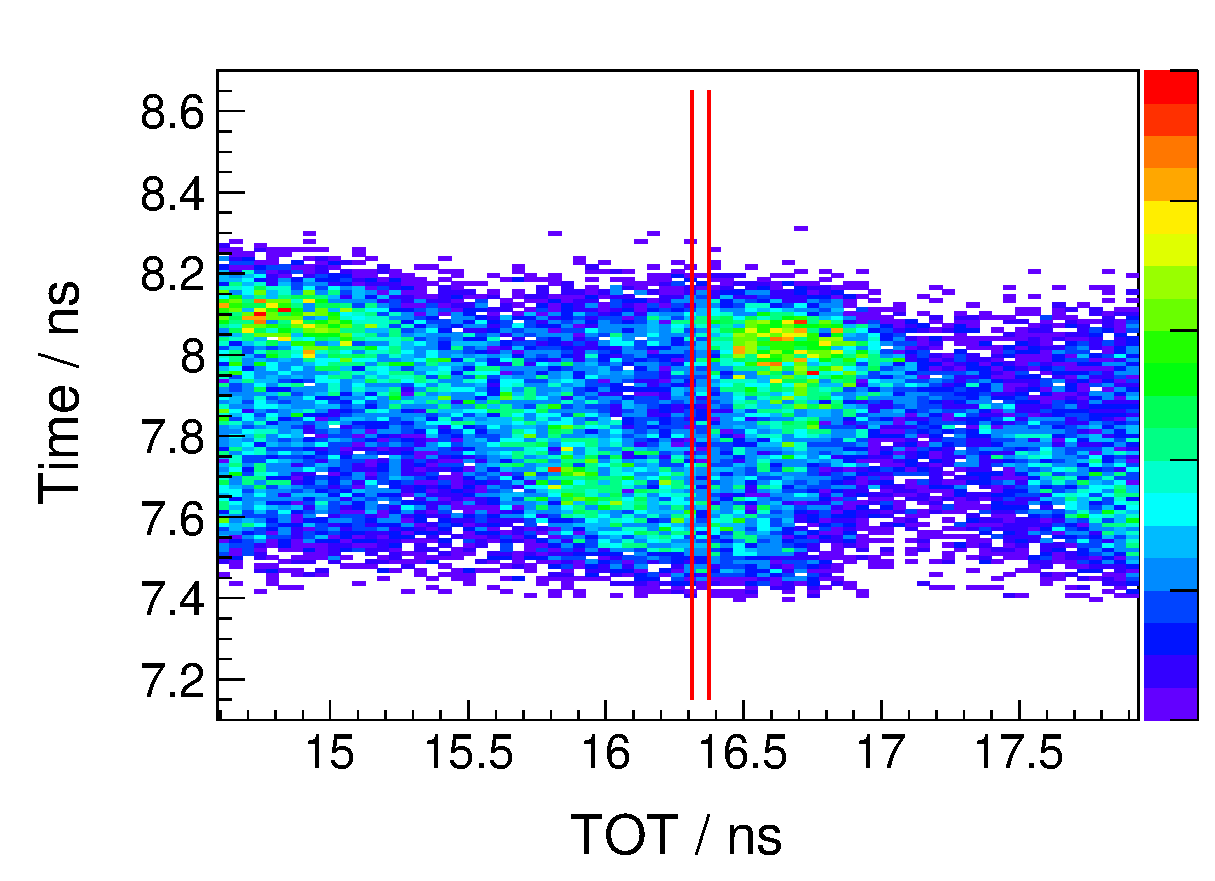
\includegraphics[width=0.9\textwidth]{chap2/cutScatterDiagram.eps}
\subcaption{截取时间对TOT的分布}
\label{fig:cutScatterDiagram}
\end{minipage}
\caption{时间对TOT的分布}
%\label{fig:Diagram}
\end{figure}

\begin{figure}[htbp]
\centering
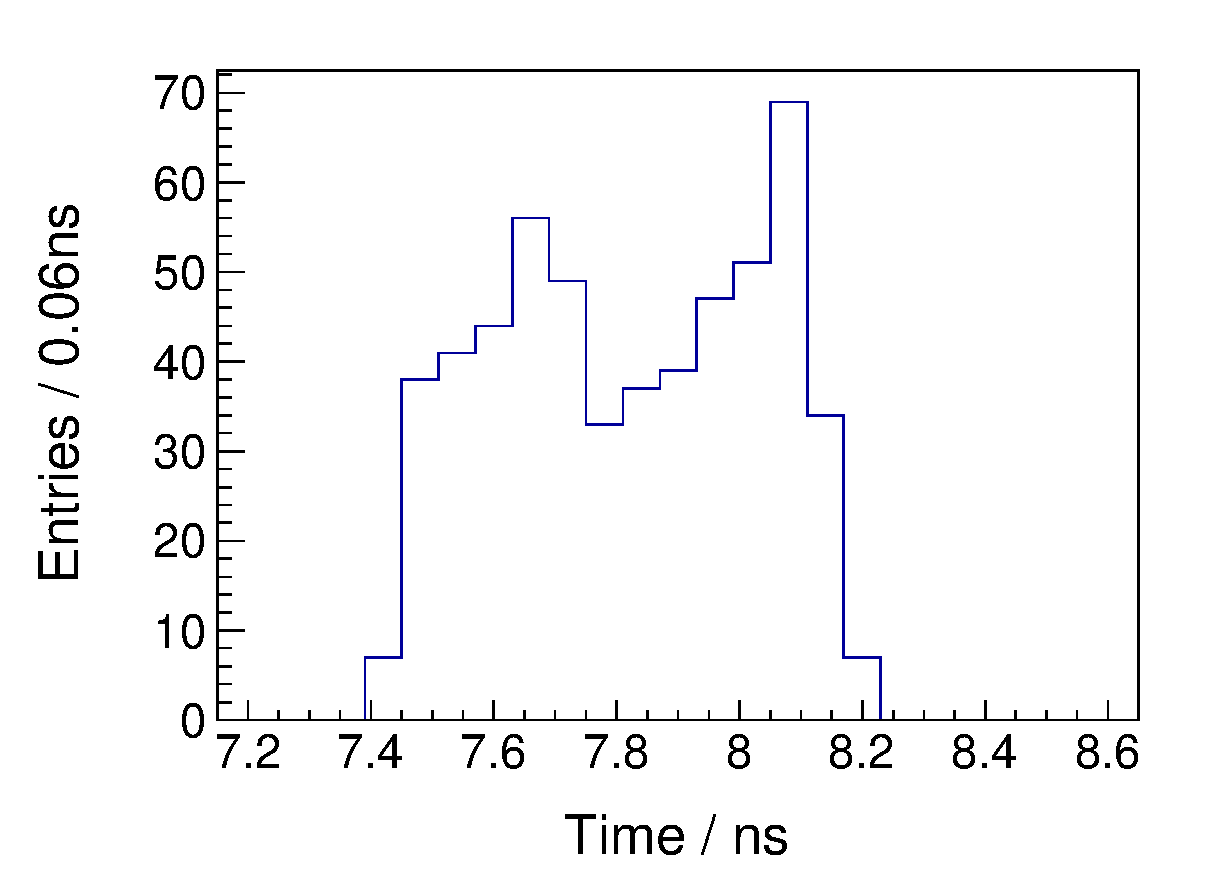
\includegraphics[width=0.5\textwidth]{chap2/onebinTime.eps}
\caption{截取一个bin的时间分布}
\label{fig:onebinTime}
\end{figure}

图~\ref{fig:onebinTime}~是一个bin内的时间分布,可以明显看出具有双峰。对此,我没有办法在一个区间内得到一个合适的中心值。

\subsection{两个高斯拟合和单个高斯拟合}

图~\ref{fig:double-ScatterDiagram}~,~\ref{fig:single-ScatterDiagram}~分布是对每个~bin~用两个高斯和一个高斯函数拟合后得到的中心值的分布

\begin{figure}[!h]
\begin{minipage}[!h]{0.5\linewidth}
%\centering
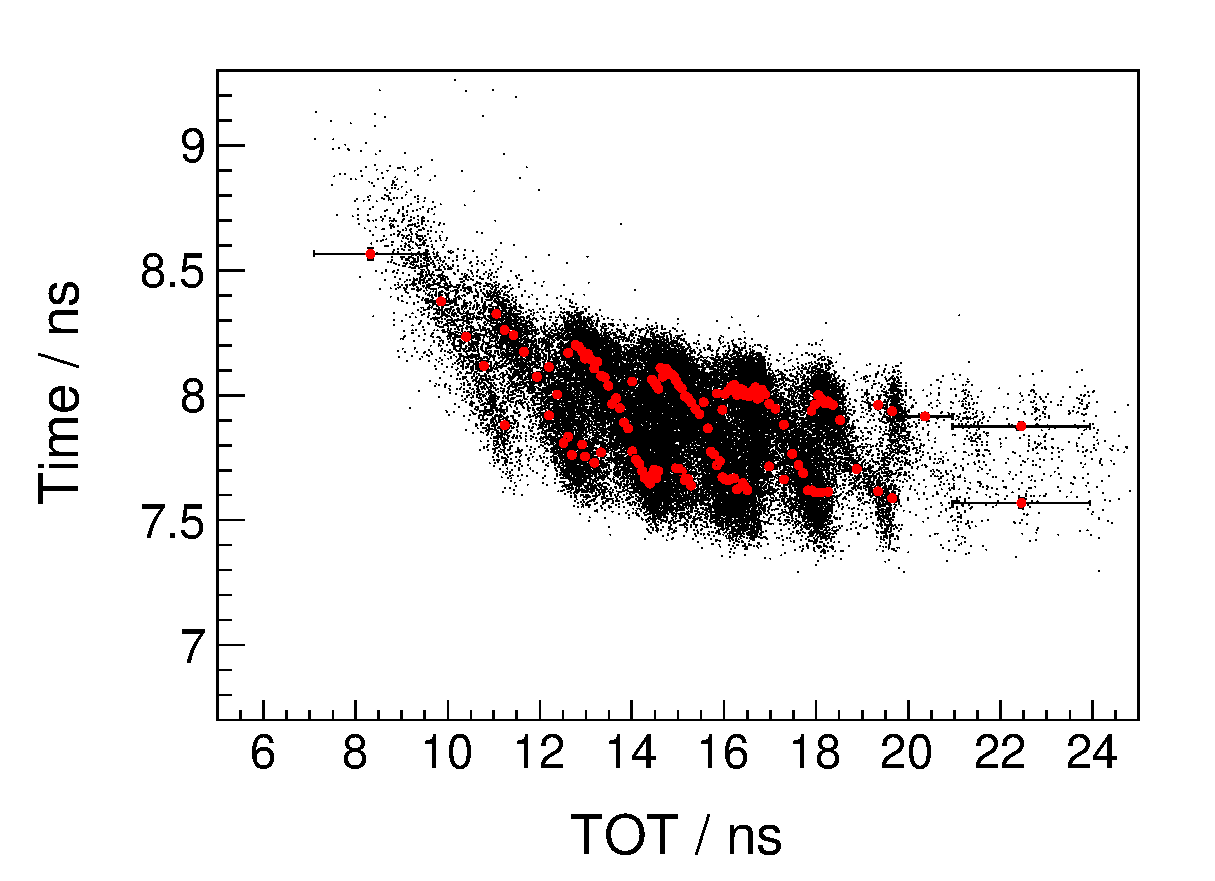
\includegraphics[width=0.95\textwidth]{chap2/double-ScatterDiagram.eps}
\subcaption{两个高斯拟合后的graph}
\label{fig:double-ScatterDiagram}
\end{minipage}%
\hfill
\begin{minipage}[!h]{0.5\linewidth}
%\centering
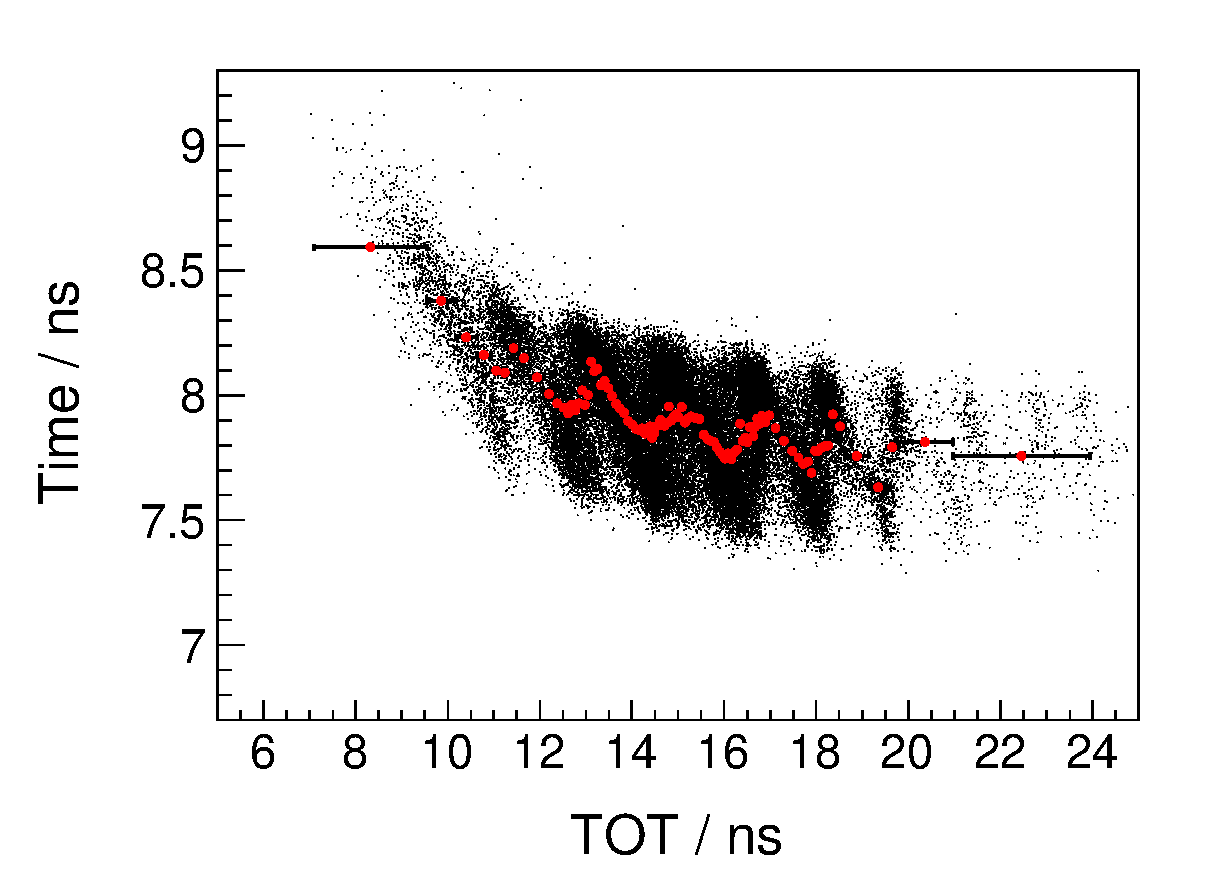
\includegraphics[width=0.95\textwidth]{chap2/single-ScatterDiagram.eps}
\subcaption{一个高斯拟合后的graph图}
\label{fig:single-ScatterDiagram}
\end{minipage}
\caption{高斯拟合后的graph}
\end{figure}

图~\ref{fig:double-leftspline}~第一种做法的样条插值曲线,每个~bin~的时间的中心值取那个比例高的。图~\ref{fig:single-leftspline}~第二种做法的样条插值曲线。可以看出,样条曲线已经把之前graph点的趋势拟合的很符合了。

\begin{figure}[!h]
\begin{minipage}[!h]{0.5\linewidth}
%\centering
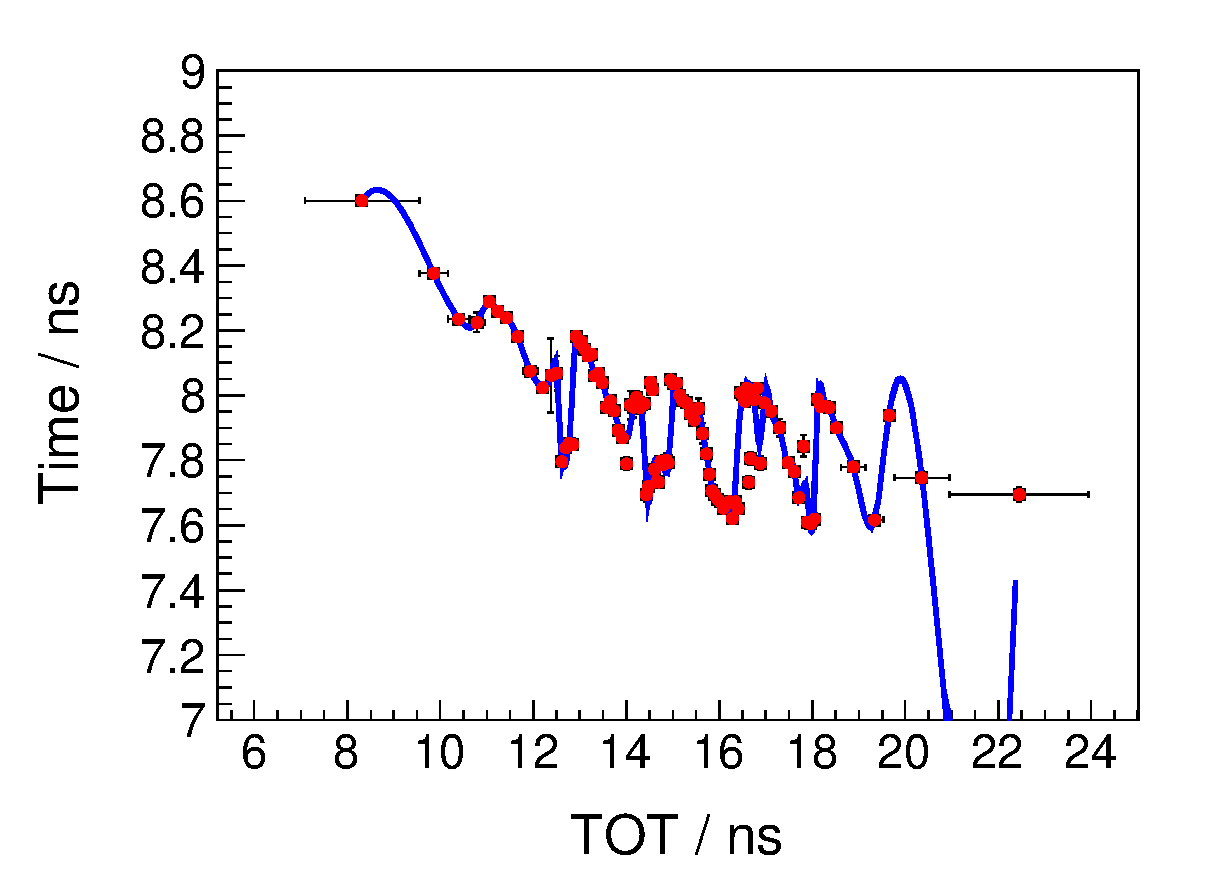
\includegraphics[width=0.95\textwidth]{chap2/double-leftspline.eps}
\subcaption{两个高斯拟合得到的中心值的样条插值}
\label{fig:double-leftspline}
\end{minipage}%
\hfill
\begin{minipage}[!h]{0.5\linewidth}
%\centering
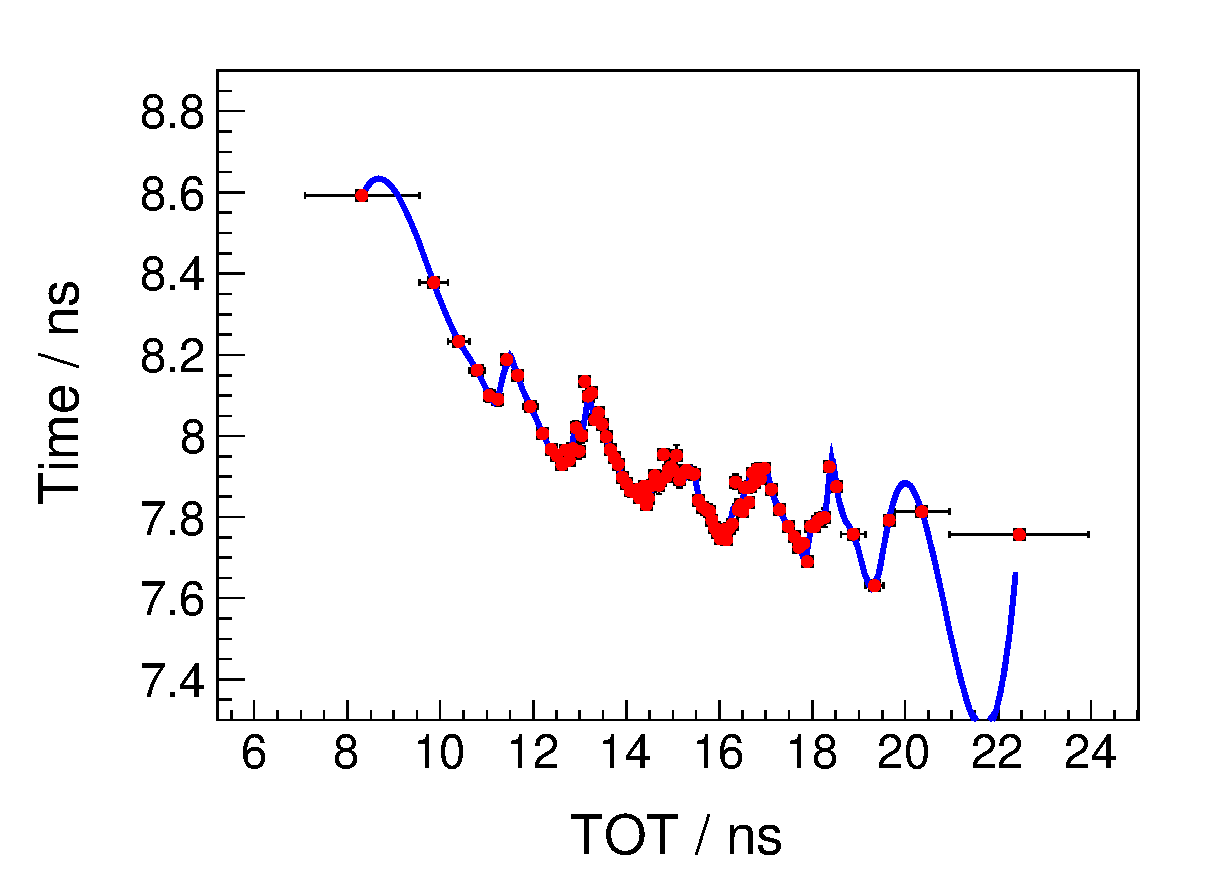
\includegraphics[width=0.95\textwidth]{chap2/single-leftspline.eps}
\subcaption{一个高斯拟合得到的中心值的样条插值}
\label{fig:single-leftspline}
\end{minipage}
\caption{样条插值}
\end{figure}

\subsection{~Z~的修正}
不管上述的哪种方法,插值修正完~TOT~后,时间随~Z~的分布都还有依赖,对此进行一个~Z~项的修正,然后得到时间分辨。图~\ref{fig:double-leftspline}~第一种做法得到的时间分辨,为~160ps~;图~\ref{fig:single-leftspline}~第二种做法得到的时间分辨,为~92ps~。

分析原因:~TOT~的多峰来自反射。一次反射内,时间对~TOT~的依赖近似线性关系,样条插值的光滑性决定不能完全描述这种关系。
\begin{figure}[!h]
\begin{minipage}[!h]{0.5\linewidth}
%\centering
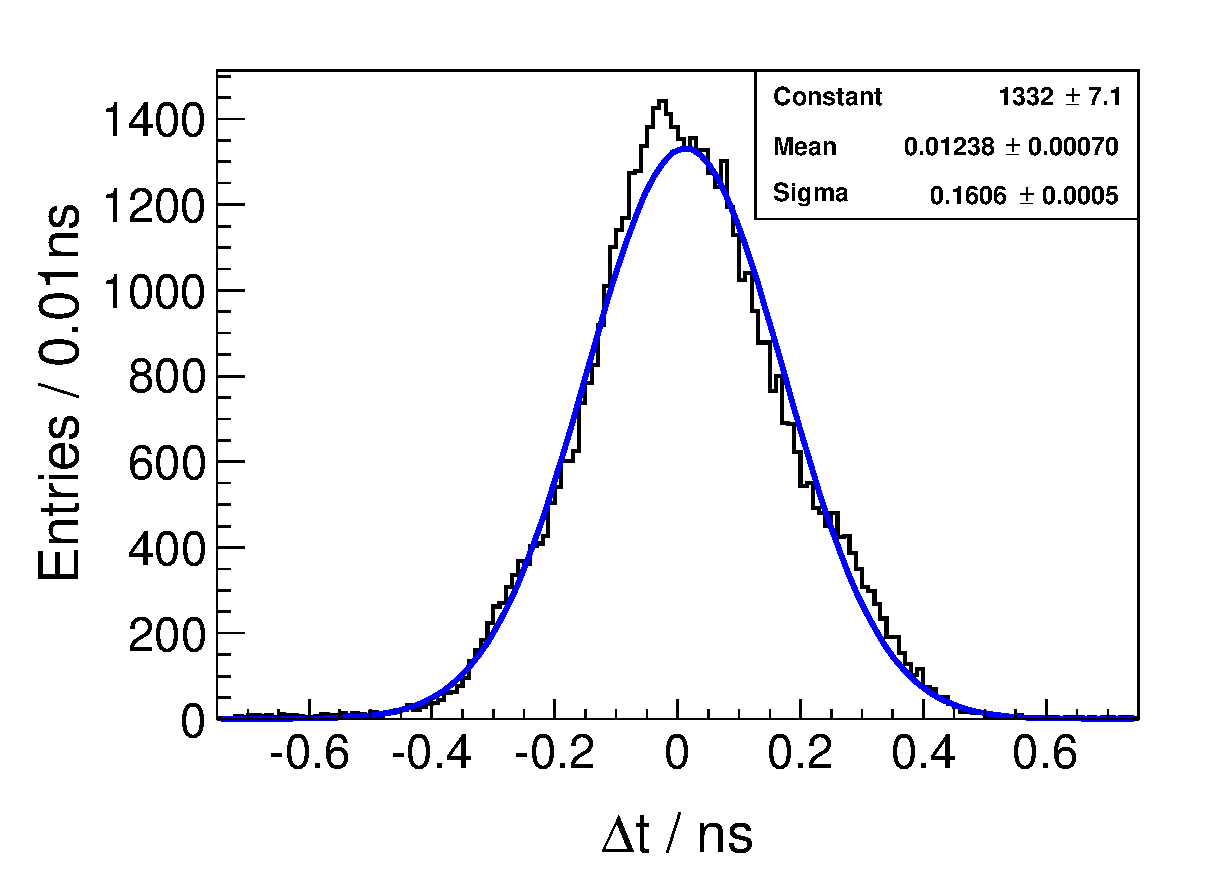
\includegraphics[width=0.8\textwidth]{chap2/double-resolutiongauss.eps}
\subcaption{时间分辨1}
\label{fig:double-resolutiongauss}
\end{minipage}%
\hfill
\begin{minipage}[!h]{0.5\linewidth}
%\centering
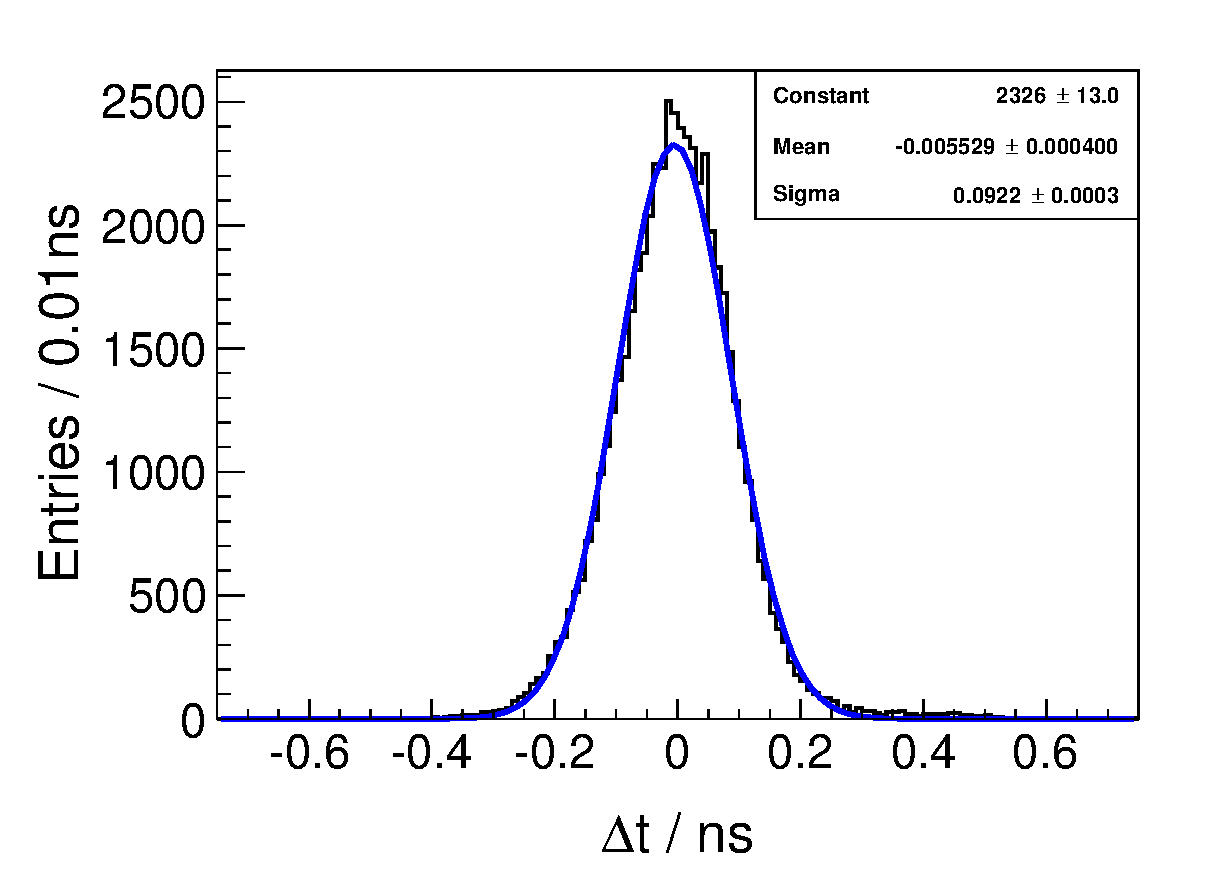
\includegraphics[width=0.8\textwidth]{chap2/single-resolutiongauss.eps}
\subcaption{时间分辨2}
\label{fig:single-resolutiongauss}
\end{minipage}
\caption{时间分辨}
\end{figure}

\subsection{反射问题}

%%%%%%%%%%%%%%%%%%%%%%%%%%%%%%%%%%%%%%%%%%%%%%%%%%%%%%%%%%%%%%%%%%%%%%%%%%%%%%%
\section{修正~Z~后进行插值}
%%%%%%%%%%%%%%%%%%%%%%%%%%%%%%%%%%%%%%%%%%%%%%%%%%%%%%%%%%%%%%%%%%%%%%%%%%%%%%

\subsection{~Z~向的修正~}
~Z~向分~bin~,然后~nov公式~拟合,最终选用三阶多项式进行拟合,修正后时间对~TOT~的依赖减弱
\subsection{插值}
分~bin~,之后进行插值,得到时间分辨
\begin{itemize}
    \item 
    \item 分bin,每个bin的时间值不唯一
    \item 对于每个bin,分别从两个高斯和一个高斯拟合
    \item 对于得到的mean值进行插值
    \item 之后对Z进行一个修正
\end{itemize}

\section{小结}
插值方法
